\chapter{Intro}\label{ch:intro}

In recent months and years, neural networks have produced many \textit{state-of-the-art} results in almost all possible disciplines of machine learning. One of the disciplines is Natural Language Processing, \textit{NLP} for short. This term covers many other hot research disciplines, including 

\begin{itemize}
\item Sentiment Analysis
\item Machine Translation
\item Voice Recognition
\item Text Generation (Neural Text Generation \textit{NTG})
\end{itemize}

Another term for text generation is denoted by \textit{Language Modelling}, because it uses the words and grammar as input for the model. In the last 5 years, there were mainly two approaches for modelling NLP, namely the rule-based system and the template-based system (Figure \ref{rules_based}). Today the \textit{State-of-the-Art} are the neural end-to-end systems, which lead to a far more advanced output \cite{End_to_End}. These new systems offer more flexibility and scale with a proportionately better results with less required data, because the complexity and thus the required computing power has increased. However, this fact leads to a complexity problem, because it becomes very difficult to understand the decisions of the neural network. The neural network is basically still a \textit{black box} to a large extent, although it gives surprisingly good results, especially in NLP. Nevertheless, neural network models for text processing are difficult to understand, so nowadays compromises between rule-based systems still have to be made and hybrid systems have to be used. 

\begin{figure}
  \begin{center}
  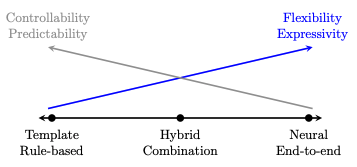
\includegraphics[width=3.5in]{photos/rule_based}\\
  \caption{Rule-Based vs. Neural-Text-Generations System \cite{End_to_End}}\label{rules_based}
  \end{center}
\end{figure}

The neural text generation, also called \textit{NTG}, has many other interesting application fields, including
\begin{itemize}
\item Speech recording and conversion to text
\item Conversation systems e.g. chatbots
\item Text summary
\end{itemize} 

In order to train language models, they must be taught the probability of occurring words in relation to the preceding words. There are several approaches to achieve this goal. Language models can be trained on the level of words, whole sentences or even whole paragraphs. The granularity in which the training takes place is called \textit{n-grams}, where \textit{n} represents the number of preceding words.

\section{Case study of a current NLP system}

\subsection{Case study}

Image-to-Text | Captionbot Microsoft

\subsection{Useful application areas of NLP systems}

IoT, Grammerly, ok

\subsection{Useful application areas of NTG systems}

Grammerly